
\subsection{Предлагаемый подход к~разработке ССМП}

Основными задачами разрабатываемой системы являются:
	\begin{ditemize}
		\item обработка входного параллельного корпуса 
			с опорой на особенности научного текста;
		\item создание моделей языка и перевода 
			на основании входного параллельного корпуса;
		\item декодирование исходного текста 
			на основании моделей языка и перевода 
				(с опорой на особенности научного текста);
		\item иметь возможность выполнять описанные выше операции распределено.
	\end{ditemize}

В соответствии с перечисленными задачами весь код системы можно разбить на 3 класса приложений, 
каждый из которых соответствует своей задаче.

\begin{figured}
		\tikzstyle{databasef} = [rectangle,thick,minimum size=1cm,draw=teal!50!black!50,top color=white,bottom color=teal!50!black!20,font=\itshape]
		\tikzstyle{readerf} = [rectangle,rounded corners,thick,minimum size=1cm,draw=blue!50!black!50,top color=white,bottom color=blue!50!black!20,font=\itshape]
		\tikzstyle{handlerf} = [rectangle,rounded corners,thick,minimum size=1cm,draw=green!50!black!50,top color=white,bottom color=green!50!black!20,font=\itshape]
		\tikzstyle{decoderf} = [rounded rectangle,thick,minimum size=1cm,draw=red!50!black!50,top color=white,bottom color=red!50!black!20,font=\itshape]
		\tikzstyle{corporaf} = [draw=yellow!50!black!70,thick,minimum height=1cm,minimum width=2cm,top color=yellow!20,bottom color=yellow!60!black!20,decorate,decoration={random steps,segment length=3pt,amplitude=1pt}]
	\begin{tikzpicture}[thick, node distance=4cm, text height=1.5ex, text depth=.25ex, auto]
		\node[databasef] 						(database)	{База данных};
		\node[readerf,above left of=database]	(reader)	{Читатель};
		\node[corporaf,left of=reader]			(corpora)	{Корпус En, Ru};
		\node[handlerf,below left of=database]	(handler)	{Обработчик};
		\node[decoderf,right of=database]		(decoder)	{Декодер};
	
		\path[->, yellow!40!black!70] 	(corpora)	edge (reader);
		\path[<-, blue] 				(database)	edge (reader);
		\path[<->, blue] 				(database)	edge (handler);
		\path[->, blue, dashed] 		(reader) 	edge (handler);
		\path[<->, red] 				(database)	edge (decoder);
	\end{tikzpicture}
	\fcaption{Упрощенная схема системы.}
\end{figured}

Кроме того, для взаимодействия с системой пользователя необходимо предусмотреть интерфейс взаимодействия 
с пользователем и с внешними приложениями. C учетом этого и условия распределенности общая 
схема может иметь вид как представлено ниже.

\begin{figured}
		\tikzstyle{databasef} = [rectangle,thick,minimum size=1cm,draw=teal!50!black!50,top color=white,bottom color=teal!50!black!20,font=\itshape]
		\tikzstyle{readerf} = [rectangle,rounded corners,thick,minimum size=1cm,draw=blue!50!black!50,top color=white,bottom color=blue!50!black!20,font=\itshape]
		\tikzstyle{handlerf} = [rectangle,rounded corners,thick,minimum size=1cm,draw=green!50!black!50,top color=white,bottom color=green!50!black!20,font=\itshape]
		\tikzstyle{decoderf} = [rounded rectangle,thick,minimum size=1cm,draw=red!50!black!50,top color=white,bottom color=red!50!black!20,font=\itshape]
		\tikzstyle{appf} = [rectangle,rounded corners,thick,minimum size=1cm,draw=orange!50!black!50,top color=white,bottom color=orange!50!black!20,font=\itshape]
		\tikzstyle{corporaf} = [draw=yellow!50!black!70,thick,minimum height=1cm,minimum width=2cm,top color=yellow!20,bottom color=yellow!60!black!20,decorate,decoration={random steps,segment length=3pt,amplitude=1pt}]
	\begin{tikzpicture}[thick, node distance=4cm, text height=1.5ex, text depth=.25ex, auto]
		\node[databasef] 						(database)	{База данных};
		\node[readerf,above left of=database]	(reader1)	{Читатель $1$};	
		\begin{scope}[node distance=2.5cm]
			\node[readerf,above right of=reader1]	(reader2)	{Читатель $2$};
			\node[readerf,above right of=reader2]	(readerd)	{Читатель $\ldots$};
			\node[readerf,above right of=readerd]	(readerx)	{Читатель $x$};
		\end{scope}
		\node[corporaf,left of=reader1]			(corpora1)	{Корпус En, Ru $1$};
		\node[corporaf,left of=reader2]			(corpora2)	{Корпус En, Ru $2$};
		\node[corporaf,left of=readerd]			(corporad)	{Корпус En, Ru $\ldots$};
		\node[corporaf,left of=readerx]			(corporax)	{Корпус En, Ru $x$};
		\node[handlerf,below left of=database]	(handler1)	{Обработчик $1$};
		\begin{scope}[node distance=2.5cm]
			\node[handlerf,below right of=handler1]	(handler2)	{Обработчик $2$};
			\node[handlerf,below right of=handler2]	(handlerd)	{Обработчик $\ldots$};
			\node[handlerf,below right of=handlerd]	(handlery)	{Обработчик $y$};
		\end{scope}
		\node[decoderf,above right of=database]		(decoder1)	{Декодер $1$};
		\node[decoderf,right of=database]			(decoder2)	{Декодер $\ldots$};
		\node[decoderf,below right of=database]		(decoder3)	{Декодер $z$};
		\begin{scope}[node distance=3.0cm]
			\node[appf,above right 	of=decoder2]		(app1)	{Web $\ldots$};
			\node[appf,right 		of=decoder2]		(app2)	{Rest $\ldots$ };
			\node[appf,below right 	of=decoder2]		(app3)	{Консоль $\ldots$ };
		\end{scope}
		\path[->, yellow!40!black!70] 	(corpora1)	edge (reader1);
		\path[->, yellow!40!black!70] 	(corpora2)	edge (reader2);
		\path[->, yellow!40!black!70] 	(corporad)	edge (readerd);
		\path[->, yellow!40!black!70] 	(corporax)	edge (readerx);
		\path[<-, blue] 				(database)	edge (reader1);
		\path[<-, blue] 				(database)	edge (reader2);
		\path[<-, blue] 				(database)	edge (readerd);
		\path[<-, blue] 				(database)	edge (readerx);
		\path[<-, blue] 				(database)	edge (handler1);
		\path[<-, blue] 				(database)	edge (handler2);
		\path[<-, blue] 				(database)	edge (handlerd);
		\path[<-, blue] 				(database)	edge (handlery);
		\path[<->, red] 				(database)	edge (decoder1);
		\path[<->, red] 				(database)	edge (decoder2);
		\path[<->, red] 				(database)	edge (decoder3);
		\path[<->, orange!50!black!50] 				(decoder2)	edge (app1);
		\path[<->, orange!50!black!50] 				(decoder2)	edge (app2);
		\path[<->, orange!50!black!50] 				(decoder2)	edge (app3);
	\end{tikzpicture}
	\fcaption{Полная схема системы.}
\end{figured}

Для эффективной работы системы предполагается, что $x < y$.
Все три типа модуля могут быть удалены географически (однако, при этом может упасть 
скорость взаимодействия). База данных может быть распределена.
Использование (возможно, удаленной) базы данных является
скорее чисто техническим моментом реализации системы. 
Намного естественнее и проще было бы проводить все вычисления в локальной памяти 
машины, а для распределения вычислений осуществлять пересылку сообщений 
от~одного узла к другому. Однако, память компьютера может быть не в состоянии
вместить все необходимые для вычисления данные даже при очень большом объеме.
А пересылка сообщений приведет к переполнению очередей сообщений для процессов,
которые медленно осуществляют обработку информации. 
На единицу времени они будут принимать больше, чем смогут обработать.
Потому самым оптимальным решением стало использование 
базы данных класса <<ключ-значение>> для каждой вычислительной 
операции, которая потребует длительного хранения.
При создании систем машинного перевода текстов с одних
естественных языков на другие возникает вопрос о том, какими
минимальными единицами смысла следует оперировать в таких
системах \cite{Хорошилов:2006}. 

Система ориентирована на перевод исключительно 
научно-технической литературы. 
Тексты научной литературы на русском и английском языках 
сходны по своей структуре.
Стиль научно-технической прозы отличается:
\begin{ditemize}
	\item устойчивыми формальными выражениями;
	\item прямым порядком слов;
	\item стереотипной структурой предложений;
	\item важностью локального порядка слов.
\end{ditemize}
Для перевода научного текста, на основании принципов изложенных в теоретической части, мы предлагаем следующие приемы:
\begin{ditemize}
	\item вместо слов использовать их группы или $n$-граммы;
	\item использовать выравнивание по крупным группам $n$-грамм;
	\item использовать модели низких порядков (IBM 3-5 могут сильно исказить локальный порядок слов).
\end{ditemize}
Как показывают статистические исследования, 
словосочетания длиной более $10$ слов 
повторяются в~текстах очень редко 
и в~совокупности покрывают их менее чем на 1\% \cite{Хорошилов:2006}.

\pagebreak

Предлагаются следующие ограничения:
{\renewcommand{\labelenumi}{\alph{enumi})}
\begin{enumerate}
	\item максимальный размер $n$-грамм положить равным $5$ слов;
	\item максимальный размер считываемой строки ограничить $256$ символами;
	\item максимальный размер предложения ограничить $40$ словами;
\end{enumerate}
}
Все эти ограничения являются настраиваемыми, однако именно 
с такими настройками проводилась реализация и тестирование системы.
Ниже рассмотрим каждое приложение в отдельности.


\subsubsection{Читатель}

\begin{figure}[H]
\begin{center}
	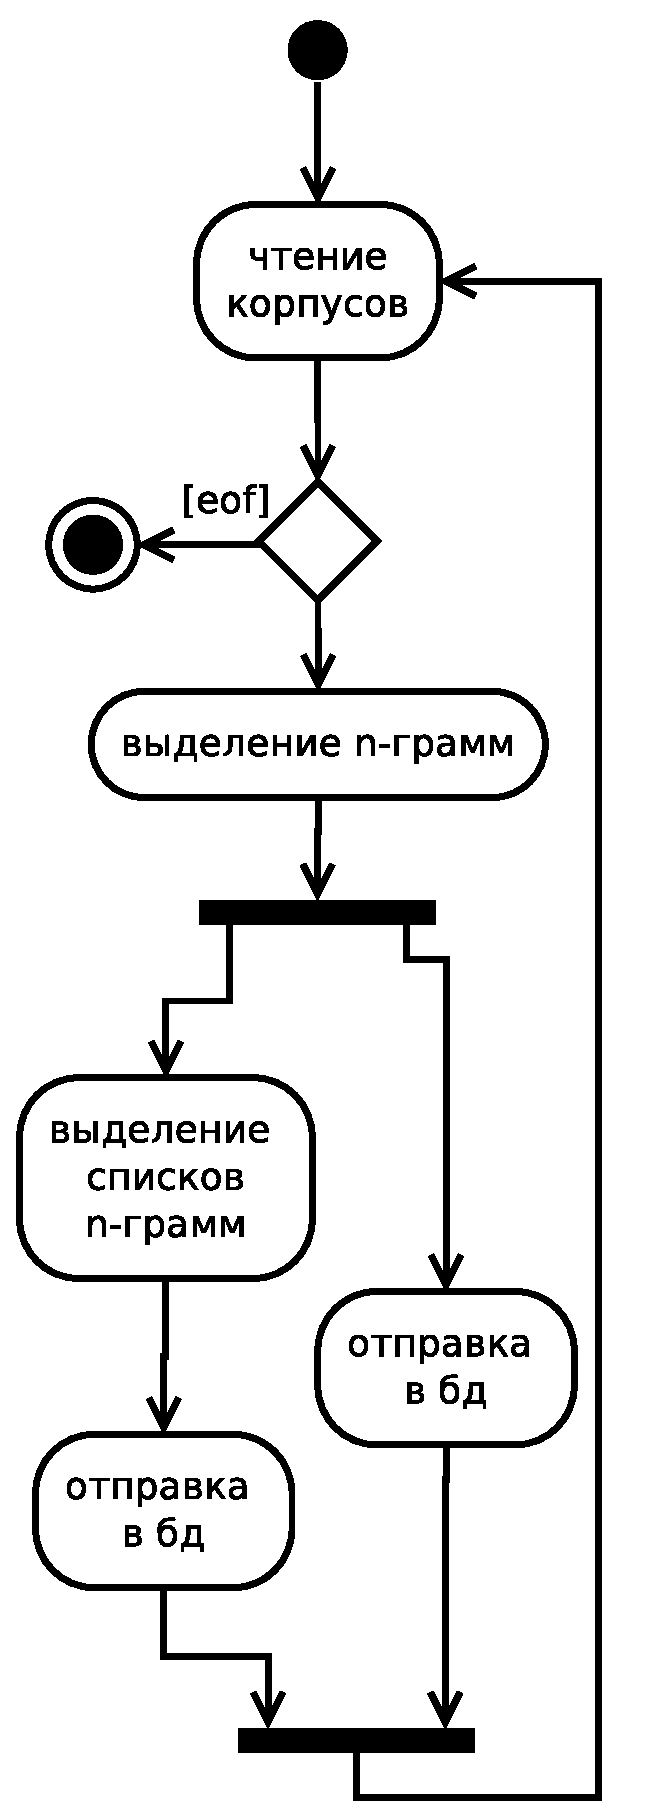
\includegraphics[height=15.0cm]{./vec/arch-reader.eps}
\end{center}
\caption{Диаграмма активности приложения <<читатель>>.}
\end{figure}

Приложение считывает параллельный корпус строка за строкой из двух файлов корпуса одновременно.
После прочтения каждая строка разбивается на слова, по синтаксическим признакам конца слова (пробелы, знаки препинания).
Из списков слов формируются группы $n$-грамм начиная с максимального $n$, 
заканчивая слова.
Одним из принципиальных моментов системы является метод выделения списков $n$-грамм.
Имея список $n$-грамм верхнего уровня, скажем пятого, составить список более низкого уровня 
можно без обращения к~исходной строке. Таким образом, выделения списка занимает время строго 
меньшее чем $O(l^2)$ по длине строки.
Формирование списков  $n$-грамм  и~отправка полученных $n$-грамм в~базу может происходить параллельно.
Сама по~себе отправка представляет собой пару операций: инкремент счетчика заданной $n$-граммы в базе 
и добавление слова множество $n$-грамм.
Обе эти операции также можно проводить параллельно, более того отправку 
в~базу данных может быть осуществлена асинхронно, так как для нас не важен возврат 
результата выполнения команды.
$n$-граммы в списке $n$-граммы отсортированы по убыванию их длин, $n$-граммы одинаковой длинны, 
отсортированы по возрастанию позиции первого слова $n$-граммы в исходном предложении.
Добавление в базу списков $n$-грамм представляет 
собой асинхронную запись каждого списка в базу данных подобно добавлению 
элемента в стек.
Общая схема приложения представлена ниже.
Стрелками показаны потоки данных.
Прерывистыми линиями изображены косвенные связи.

\begin{figured}
		\tikzstyle{dspf} = [rectangle,thick,minimum size=1cm,draw=teal!50!black!50,top color=white,bottom color=teal!50!black!20,font=\itshape]
		\tikzstyle{filef} = [rectangle,rounded corners,thick,minimum size=2.5cm,draw=blue!50!black!50,top color=white,bottom color=blue!50!black!20,font=\itshape]
		\tikzstyle{handlerf} = [rectangle,rounded corners,thick,minimum size=2cm,draw=green!50!black!50,top color=white,bottom color=green!50!black!20,font=\itshape]
		\tikzstyle{dbf} = [rounded rectangle,thick,minimum size=2cm,draw=red!50!black!50,top color=white,bottom color=red!50!black!20,font=\itshape]
		
		\tikzstyle{dbpoolf} = [rounded rectangle,thick,minimum size=1cm,draw=orange!50!black!50,top color=white,bottom color=orange!50!black!20,font=\itshape]
		
		\tikzstyle{dbconf} = [rounded rectangle,thick,minimum size=1cm,draw=orange!50!black!50,top color=white,bottom color=orange!50!black!20,font=\itshape]

		\tikzstyle{corporaf} = [draw=yellow!50!black!70,thick,minimum height=1cm,minimum width=2cm,top color=yellow!20,bottom color=yellow!60!black!20,decorate,decoration={random steps,segment length=3pt,amplitude=1pt}]
	\begin{tikzpicture}[thick, node distance=4cm, text height=1.5ex, text depth=.25ex, auto]
		\node[dspf] 						(dsp)	{Диспетчер};
		\node[filef,	above left of=dsp]	(file)
		{
			\begin{tabular}{c}
				Обработчик 	\\ 
				файлов 	\\ 
				(потоков) 	\\ 
			\end{tabular} 
		};
		\node[corporaf,	left of=file]			(corpora)	{Корпус En, Ru};
		\node[handlerf,	above right of=dsp]	(handler)	
		{
			\begin{tabular}{c}
				Модуль работы	\\ 
				со словами		\\ 
			\end{tabular} 
		};
		\node[dbf,	below right of=dsp]		(db)
		{
			\begin{tabular}{c}
				Модуль \\ 
				работы с БД	\\ 
			\end{tabular} 
		};
		\node[dbpoolf,	below left of=dsp]		(dbpool) {Пул соединений};
		\path[->, yellow!40!black!70] 	(corpora)	edge (file);
		\path[<-, blue] 				(dsp)	edge (file);
		\path[<->, blue] 				(dsp)	edge (handler);
		\path[->, red, dashed] 		(file) 	edge (handler);
		\path[->, blue] 				(dsp)	edge (db);
		\path[->, red, dashed] 		(handler) 	edge (db);
		\path[->, blue] 				(db)	edge (dbpool);
	\end{tikzpicture}
	\fcaption{Схема модулей приложения <<читатель>>. }
\end{figured}

В одной из модификаций этого приложения мы сразу в приложении читателя составляли список сопоставления
$n$-грамм разных языков. Это позволяло несколько разгрузить приложение обработчика кроме того давало
возможность гибко настраивать сопоставление $n$-грамм разного размера.

Полный список сопоставления $n$-грамм представляет собой декартово произведения списков $n$-грамм
на разных языках. Но использование полного списка для $n$-грамм  большого размера является 
не экономичным с точки зрения хранения информации. Тем более, учитывая, стилистические особенности
научного текста, крупные группы слов отражающие сходные понятия в научных текстах находятся
примерно на одинаковом удалении от начала предложения.

Для этого случая нами был разработан следующий подход:
{\renewcommand{\labelenumi}{\alph{enumi})}
	\begin{enumerate}
		\item строить полный список сопоставлений (декартово произведение) для $1$-грамм, то есть слов;
		\item строить $m$-диагональную матрицу для всех остальных $n$-грамм.
	\end{enumerate}
}
$m$ выбирается экспериментально, по умолчанию полагается равным $3$.
Такой подход позволяет снизить количество сопоставляемых $n$-грамм, но повышает вероятность
ошибки обучения системы. 
Как показала практика, не все научные тексты удовлетворяют ограничению представленному выше.
Кроме того, это предположение является ошибочным для текстов иных стилей.
В текущей реализации мы отказались от такого подхода.

\pagebreak

\subsubsection{Обработчик}
Обработчик нужен для обучения модели перевода на основании данных полученных у читателя.

\begin{figure}[H]
	\begin{center}
		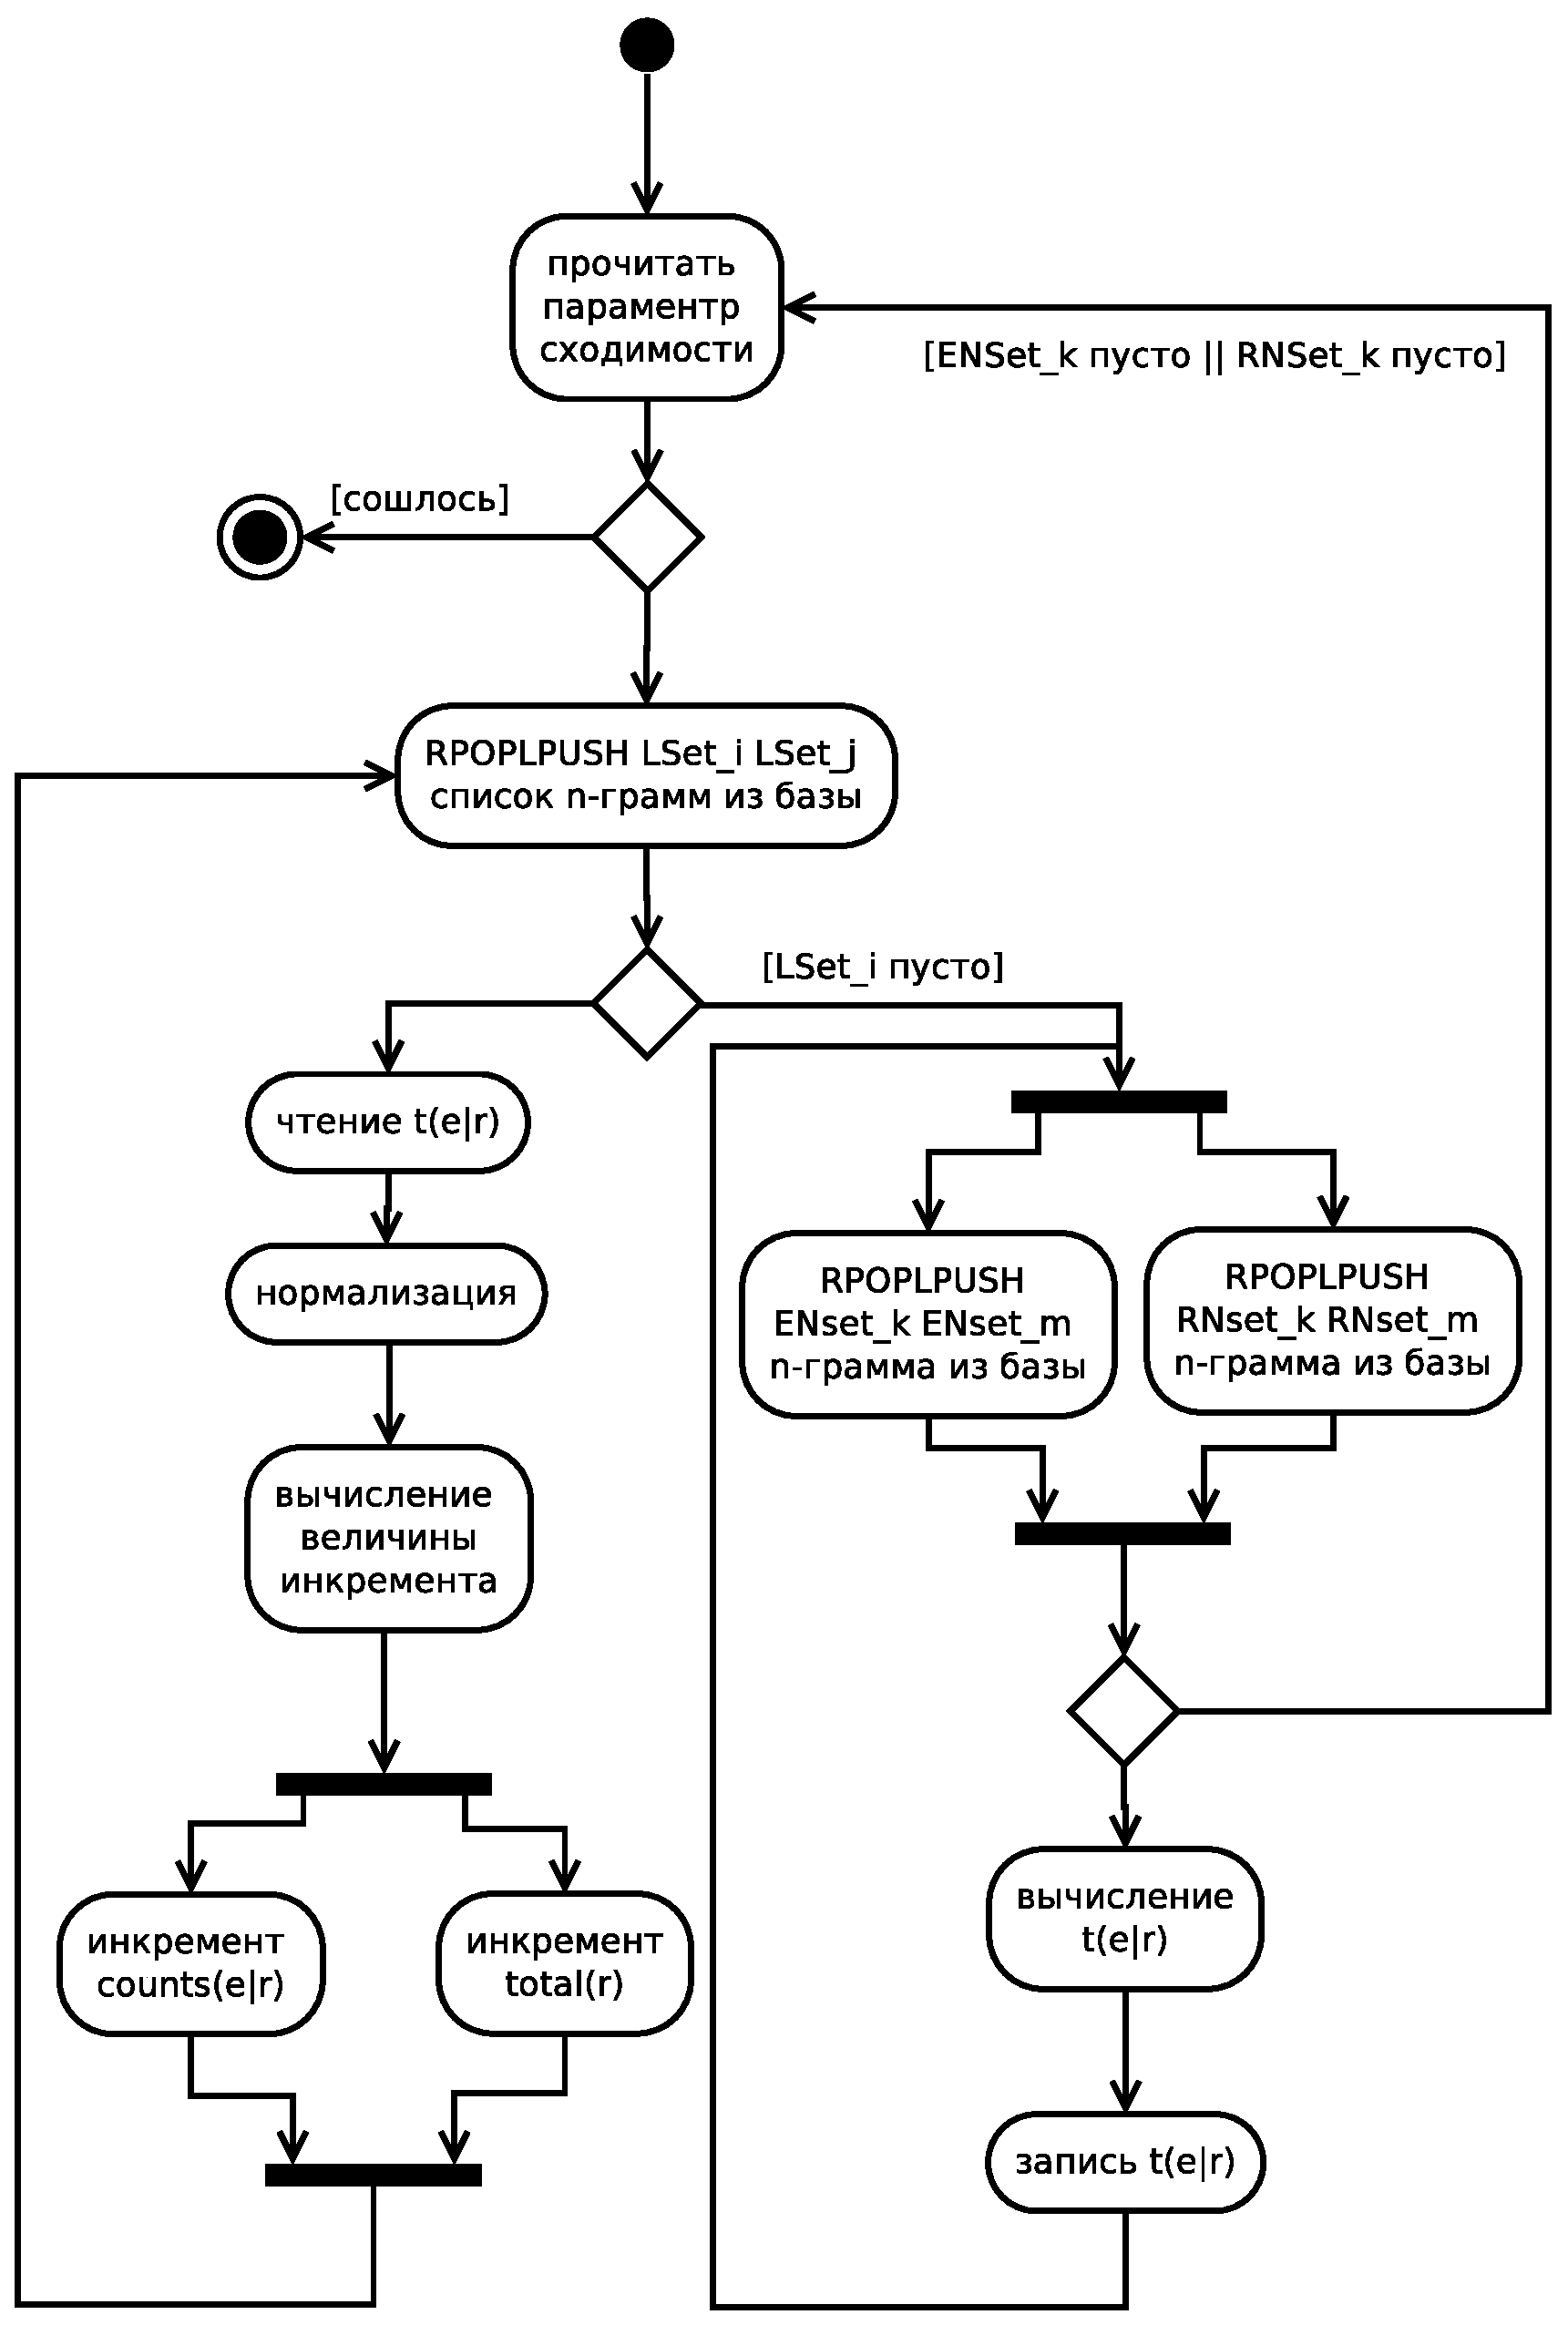
\includegraphics[height=18.0cm]{./vec/arch-handler.eps}
	\end{center}
	\caption{Диаграмма активности приложения <<обработчик>>.}
\end{figure}

\pagebreak

Принцип работы обработчика во многом определяется алгоритмом обучения описанным 
в выше. 
Условие сходимости предлагается не вычислять как математическое неравенство.
Как показала практика на текстах ограниченного объема это условие может никогда не выполниться,
тем более нам не столь важен сам факт сходимости, сколько относительные отношения вероятностей
парных соответствий $n$-грамм. 

Важными архитектурными моментами работы приложения 
являются методы доступа к данным. 
Предполагается что все операции на запись данных буду асинхронными.
Операция инкремента величины подсчетов (см. алгоритмы в приложении),
должны быть атомарными и асинхронными. В противном случае, 
если мы используем распределенные вычисления, то данные рискуют быть 
или неверно прочитаны или перезаписаны в неподходящий момент (оптимистическая блокировка).
Использование пессимистической блокировки может привести 
к значительному замедлению при большой конкуренции запросов.

$\mathrm{Lset}_0$ --- пары списков $n$-грамм перемещенные туда читателем.
На момент начала работы обработчика предполагается что это множество не пусто.
На каждом проходе по множеству элемент этого множества считывается в обработчик
и перемещается в $\mathrm{Lset}_1$ (это выполняется как атомарная операция {\tt rpoplpush}).
При каждой $i$-й итерации алгоритма обработчик считывает 
пару списков $n$-грамм из $\mathrm{Lset}_0$ и кладет их в множество $\mathrm{Lset}_{i+1}$.
Ситуация с вычислением вероятности по всем $n$-граммам корпуса аналогична,
за исключением того, что считывание и перемещение ведется сразу по двум множествам.
Тут так же предполагается, что используемая база данных поддерживает 
атомарные операции такого вида.
В противном случае могут возникнуть конфликты записи данных
и есть возможность, что алгоритм будет многократно отрабатывать 
с ограниченным объемом одних и тех же данных.

Использование множеств в данном контексте может показаться странным.
Более того, оно может показать не самым эффективным решением.
Однако это не так. 
Выбор терминологии и структур хранения данных 
был сделан из практических соображений.
В ходе проектирования и промежуточных реализаций системы 
было опробовано много различных вариантов, которые описаны в ниже.

\pagebreak

\begin{figured}
		\tikzstyle{dspf} = [rectangle,thick,minimum size=1cm,draw=teal!50!black!50,top color=white,bottom color=teal!50!black!20,font=\itshape]
		\tikzstyle{filef} = [rectangle,rounded corners,thick,minimum size=2.5cm,draw=blue!50!black!50,top color=white,bottom color=blue!50!black!20,font=\itshape]
		\tikzstyle{handlerf} = [rectangle,rounded corners,thick,minimum size=2cm,draw=green!50!black!50,top color=white,bottom color=green!50!black!20,font=\itshape]
		\tikzstyle{dbf} = [rounded rectangle,thick,minimum size=2cm,draw=red!50!black!50,top color=white,bottom color=red!50!black!20,font=\itshape]
		\tikzstyle{dbpoolf} = [rounded rectangle,thick,minimum size=1cm,draw=orange!50!black!50,top color=white,bottom color=orange!50!black!20,font=\itshape]
		\tikzstyle{dbconf} = [rounded rectangle,thick,minimum size=1cm,draw=orange!50!black!50,top color=white,bottom color=orange!50!black!20,font=\itshape]
		\tikzstyle{corporaf} = [draw=yellow!50!black!70,thick,minimum height=1cm,minimum width=2cm,top color=yellow!20,bottom color=yellow!60!black!20,decorate,decoration={random steps,segment length=3pt,amplitude=1pt}]
	\begin{tikzpicture}[thick, node distance=4cm, text height=1.5ex, text depth=.25ex, auto]
		\node[dspf] 						(dsp)	{Диспетчер};
		\node[handlerf,	above right of=dsp]	(handler)	
		{
			\begin{tabular}{c}
				Вычислительный 	\\ 
				модуль			\\ 
			\end{tabular} 
		};
			\node[filef,	above left of=handler]	(cnt)
				{
					\begin{tabular}{c}
						Вычисление  \\ 
						подсчетов	\\ 
					\end{tabular} 
				};
			\node[filef,	above right of=handler]	(t)
				{
					\begin{tabular}{c}
						Вычисление	\\ 
						$t(\WE|\WR)$	\\ 
					\end{tabular} 
				};
		\node[dbf,	above left of=dsp]		(db)
		{
			\begin{tabular}{c}
				Модуль \\ 
				работы с БД	\\ 
			\end{tabular} 
		};
		\node[dbpoolf,	below left of=db]		(dbpool) {Пул соединений};
		\path[<->, blue] 				(dsp)	edge (handler);
		\path[<->, blue] 				(dsp)	edge (db);
		\path[<->, red, dashed] 		(handler) 	edge (db);
		\path[<->, blue] 				(db)	edge (dbpool);
		\path[<->, blue] 		(handler) 	edge (cnt);
		\path[<->, blue] 		(handler) 	edge (t);
	\end{tikzpicture}
	\fcaption{Схема модулей приложения <<обработчик>>.}
\end{figured}

Выше представлена схема модулей приложения обработчика.
Стрелками показаны потоки данных.
Прерывистыми линиями изображены косвенные связи.

Для системы крайне критично время доступа к базе данных,
так как для всех численных операций база используется 
как временное хранилище данных между итерациями алгоритма обучения.
Именно поэтому мы на архитектурной схеме изображаем
такую техническую деталь как пул соединений.

\pagebreak

\subsubsection{Декодер}

Согласно описанному ранее алгоритму жадного инкрементного 
поиска декодер имеет два режима работы.

В первом режиме работы на вход принимается исходный текст.
Далее ищется ее наиболее вероятный эквивалент, последовательным разбиением 
фразы на $n$-граммы наибольшего размера (аналогично алгоритму системы перевода основанной на примерах в приложении), 
и параллельным поиском их в базе данных.
После того, как эквивалент всего текста был найден, вычисляется 
величина неопределенности текста:

\begin{Large}
\[
	\text{ВН} = 2^{- \left( \frac{1}{S_{\NE}}\sum\limits_{i = 1}^{S_{\NE}} \log_2 P(\NE_i) 
		+ \frac{1}{S_{\WE}}\sum\limits_{j = 1}^{S_{\WE}} \log_2 P(\WR_j|\WE_j) \right) } 
\]
\end{Large}

\begin{itemize}
	\item $\NE$ --- $n$-граммы высокого порядка найденные в созданном тексте;
	\item $S_{\NE}$ --- количество таких $n$-грамм;
	\item $P(\NE)$ --- вероятность $n$-грамм согласно языковой модели (вычисляется как указано раннее);
	\item $\WE$ --- $n$-граммы (слова) как результат перевода согласно модели перевода;
	\item $S_{\WE}$ --- количество таких $n$-грамм (слов);
	\item $P(\WR_j|\WE_j)$ --- вероятность перевода фразы $\WE_j$ на $\WR_j$.
\end{itemize}

Во втором режиме работы на вход принимается исходный текст (ИТ), переводной текст (ПТ)
c предыдущей итерации и величина неопределенности (ВН).
Применяются операции описанные выше для алгоритма жадного инкрементного поиска,
если полученное новое значение имеет меньшую величину неопределенности чем предыдущее,
то оно подается на выход. В~противном случае итерации продолжаются.

Интерфейсная часть декодера представляет собой 
набор отдельных приложений, которые вызывают функции декодера при поступлении 
запросов на перевод. Общая схема декодера представлена ниже.
Стрелками показаны потоки данных.
Прерывистыми линиями изображены косвенные связи.

\begin{figure}[H]
\begin{center}
		\tikzstyle{dspf} = [rectangle,thick,minimum size=1cm,draw=teal!50!black!50,top color=white,bottom color=teal!50!black!20,font=\itshape]
		\tikzstyle{filef} = [rectangle,rounded corners,thick,minimum size=2.5cm,draw=blue!50!black!50,top color=white,bottom color=blue!50!black!20,font=\itshape]
		\tikzstyle{handlerf} = [rectangle,rounded corners,thick,minimum size=2cm,draw=green!50!black!50,top color=white,bottom color=green!50!black!20,font=\itshape]
		\tikzstyle{dbf} = [rounded rectangle,thick,minimum size=2cm,draw=red!50!black!50,top color=white,bottom color=red!50!black!20,font=\itshape]
		\tikzstyle{dbpoolf} = [rounded rectangle,thick,minimum size=1cm,draw=orange!50!black!50,top color=white,bottom color=orange!50!black!20,font=\itshape]
		\tikzstyle{dbconf} = [rounded rectangle,thick,minimum size=1cm,draw=orange!50!black!50,top color=white,bottom color=orange!50!black!20,font=\itshape]
		\tikzstyle{corporaf} = [draw=yellow!50!black!70,thick,minimum height=1cm,minimum width=2cm,top color=yellow!20,bottom color=yellow!60!black!20,decorate,decoration={random steps,segment length=3pt,amplitude=1pt}]
	\begin{tikzpicture}[thick, node distance=4cm, text height=1.5ex, text depth=.25ex, auto]
		\node[dspf] 						(dsp)	{Диспетчер};
		\begin{scope}[node distance=3.0cm]
		\node[handlerf, above of=dsp]	(iface)	
		{
			\begin{tabular}{c}
				Интерфейсный 	\\ 
				модуль			\\ 
			\end{tabular} 
		};
		\end{scope}			

			\node[handlerf, above left of=iface]	(web)	
			{
				\begin{tabular}{c}
					Веб 				\\ 
					приложение			\\ 
				\end{tabular} 
			};
			
			%	\node[dbpoolf,	above left of=web]		(webctl) {Контроллеры};
			%	\node[dbpoolf,	above right of=web]		(url) {Обработчик URL};
			%	\node[dbpoolf,	left of=web]			(webtpl) {Шаблоны};
			%	\node[dbpoolf,	below left of=web]		(webxsl) {XSLT-преобразователь};
			\node[handlerf, above right of=iface]		(rest)	
			{
				\begin{tabular}{c}
					Rest 	\\ 
					приложение	\\ 
				\end{tabular} 
			};
			%	\node[dbpoolf,	above right of=rest]		(restctl) {Контроллеры};
		\node[handlerf, below right of=dsp]	(handler)	
		{
			\begin{tabular}{c}
				Вычислительный 	\\ 
				модуль			\\ 
			\end{tabular} 
		};
			\node[filef, below left of=handler]	(cnt)
				{
					\begin{tabular}{c}
						Начальный  \\ 
						перевод	\\ 
					\end{tabular} 
				};
			\node[filef, below right of=handler]	(t)
				{
					\begin{tabular}{c}
						Улучшение \\ 
						перевода \\ 
					\end{tabular} 
				};
		\node[dbf, below left of=dsp]		(db)
		{
			\begin{tabular}{c}
				Модуль \\ 
				работы с БД	\\ 
			\end{tabular} 
		};
		\node[dbpoolf,	below left of=db]		(dbpool) {Пул соединений};

		\path[<->, blue] 				(dsp)	edge (handler);
		\path[<->, blue] 				(dsp)	edge (db);
		\path[<->, red, dashed] 		(handler) 	edge (db);
		\path[<->, blue] 				(db)	edge (dbpool);
		\path[<->, blue] 		(handler) 	edge (cnt);
		\path[<->, blue] 		(handler) 	edge (t);
		\path[<->, red, dashed] 		(iface.west) edge (db);
		\path[<->, red, dashed] 		(iface.east) edge (handler);
		\path[<->, blue] 				(iface)	edge (dsp);
		\path[<->, blue] 				(iface)	edge (web);
		\path[<->, blue] 				(iface)	edge (rest);
		% \path[<->, blue] 				(webctl)	edge (web);
		% \path[->, blue] 				(webtpl)	edge (web);
		% \path[<->, blue] 				(webxsl)	edge (web);
		% \path[->, blue] 				(url)	edge (web);
		% \path[->, blue] 				(url)	edge (rest);
		% \path[<->, blue] 				(restctl)	edge (rest);
		% \path[<-, red, dashed] 		(restctl) edge (url);
		% \path[<-, red, dashed] 		(webctl) edge (url);
	\end{tikzpicture}
\end{center}
\caption{Схема модулей приложения <<декодер>>.}
\end{figure}

Rest-приложение представляет из себя HTTP RESTful веб-службу.
К ней по определенному адресу поступает HTTP запрос POST вида.
В теле запроса передается исходный текст для перевода,
который отправляется для декодирования.
После первой итерации декодирования Rest-приложение, 
отвечает запросившему клиенту первым <<наихудшим>> вариантом перевода.
Далее не разрывая соединения генерируются другие варианты перевода
и сразу передаются клиенту. Это продолжается пока клиент 
самостоятельно не разорвет соединение.

Веб-приложение представляет из себя обычный веб-ресурс,
где пользователю предлагается ввести исходный текст для перевода.
После осуществления первой итерации перевода, пользователю
будет предложено улучшить полученный вариант перевода.
Количество итераций по улучшению перевода определяет 
в данном случае сам пользователь.


\begin{figure}[H]
	\begin{center}
		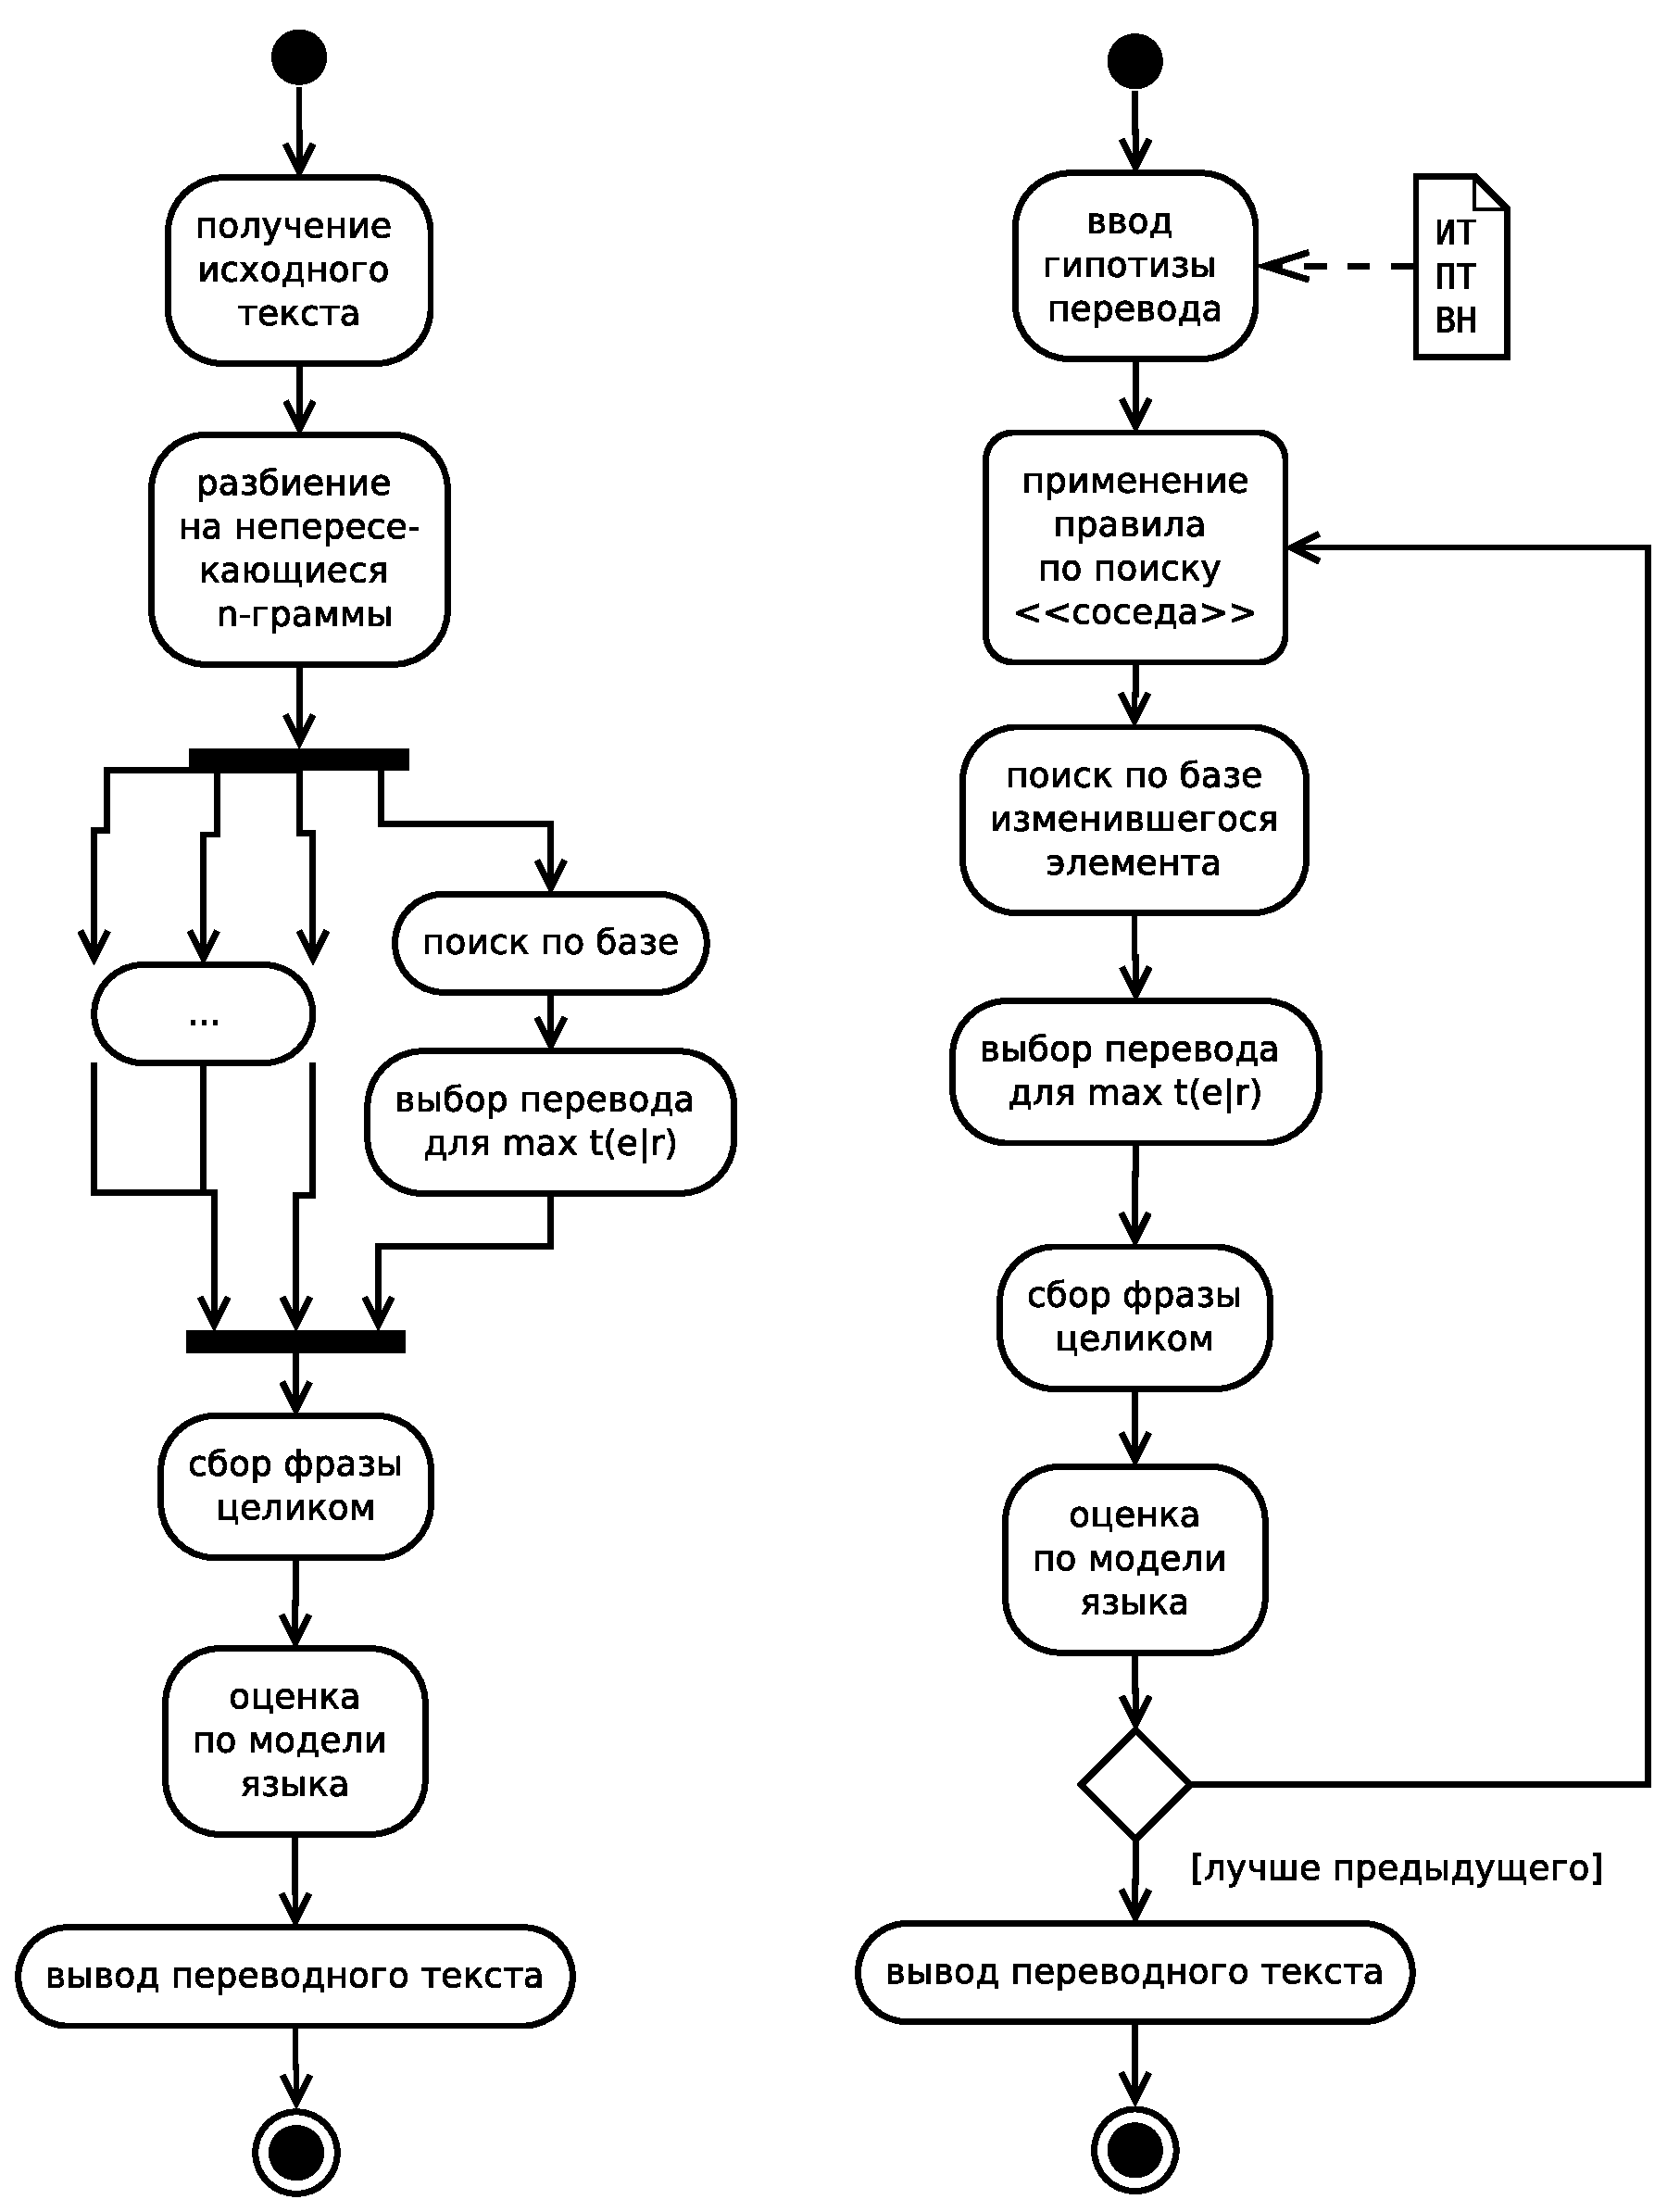
\includegraphics[height=18.0cm]{./vec/arch-decoder.eps}
	\end{center}
	\caption{Диаграммы активности приложения <<декодер>>.}
\end{figure}


\pagebreak

